\chapter{Applications}
This chapter will introduce mathematically some applications which are using  Hawkes process.
\section{Seismic Events}
In reality, the earthquakes regularly occur. To decrease the risk and damage, Alan Hawkes introduced some probability models to predict the occurrence of large earthquakes. The epidemic type aftershock sequence model is a particular type of marked Hawkes process for modeling earthquake times and magnitudes. This model can be defined by its intensity

$$\lambda(t) = \lambda_{0} + \alpha \sum_{t_{i} < t} e^{\delta\kappa_{i}} e^{-\beta(t-t_{i})}.$$
where $\alpha, \beta, \delta > 0 $ are parameters, with an exponential distribution as its mark density  and $\kappa_{i} \in [0, \infty)$ denotes the magnitude of an earthquake occurring
at time $t_{i}.$
$$f(\kappa|t) = \gamma e^{-\gamma\kappa}.$$
The conditional intensity function including both marks and times is
$$\lambda(t,\kappa) =( \lambda_{0} + \alpha \sum_{t_{i} < t} e^{\delta\kappa_{i}} e^{-\beta(t-t_{i})})\gamma e^{-\gamma\kappa}.$$

 \begin{figure}[H]
 	\centering
 	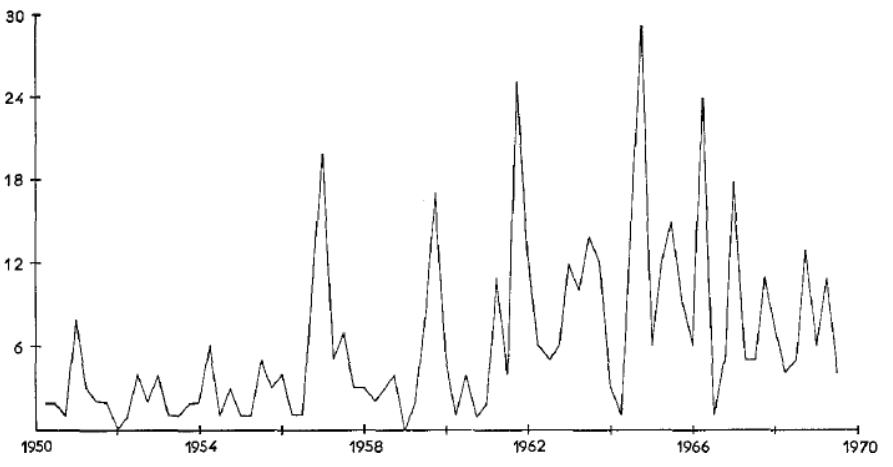
\includegraphics[width=0.8\textwidth ]{Application_Seismic.PNG}
 	\caption{The number of shocks in periods of three months for an area of the North Atlantic (refer to \cite{HawkesProcesses_KatarzynaObral}).}
 	\label{Application_Seismic}
 \end{figure}

Seeing in Figure \ref{Application_Seismic} that the number of shocks in periods of three months for an area of the North
Atlantic resembles the stochastic intensity function of a Hawkes process.

\section{Risk Process with Hawkes Process}
In insurance field, the risk estimation is important. Hence Stabile and Torrisi consider risk processes with non-stationary Hawkes claims arrivals. They introduce the following risk model for the surplus process (risk process)
$$ U(t,x) = x + ct - \displaystyle\sum_{i=1}^{N(t)}Z_{i}$$
where ${N(t), t \geq 0} $ is the number of points of a non-stationary Hawkes process, in the time interval $(0, t]$, $x$, $c > 0$ and $\{Z_{i}, i = 1, 2, . . .\}$ are the same as for the classic model.

 \begin{figure}[H]
 	\centering
 	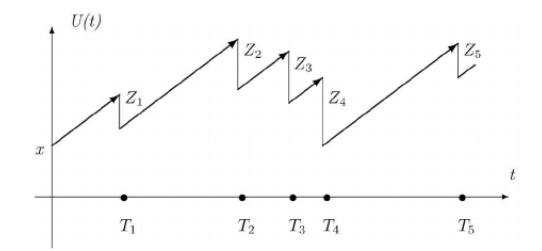
\includegraphics[width=0.8\textwidth ]{SurplusProcess.PNG}
 	\caption{Behavior of the surplus process (refer to \cite{SurplusProcess}).}
 	\label{Surplus_Process}
 \end{figure}
 The interpretation of the risk model is the following: the
 standard claims which occur according to the immigrant-points trigger claims according
 to the branching structure. Typically, the fertility rate of an immigrant is taken to
 be monotonic decreasing, meaning that the claim number process has a self-exciting
 structure in which recent events affect the intensity of claim occurrences more than
 distant ones.
